
%%%%%%%%%%%%%%%%%%%%%%%%%%%%%%%%%%%%%%%%%%%%%%%%%%%%%%%%%%%%%%%%%%%%%%%%%%%%%%%%%
% Document template TEX-STD-A4 by g0hl1n
%
% This document is derived from the TEX-STD-A4 template.
% The TEX-STD-A4 template was released into the public domain.
% For more information, please refer to <http://unlicense.org/>
%   Template-Source:  https://github.com/g0hl1n/LaTeX
%   Template-Author:  Richard 'g0hl1n' Leitner <me@g0hl1n.net>
%   Template-Version: 1.1
%%%%%%%%%%%%%%%%%%%%%%%%%%%%%%%%%%%%%%%%%%%%%%%%%%%%%%%%%%%%%%%%%%%%%%%%%%%%%%%%%
\documentclass[a4paper,12pt]{article} % An article on a4paper with 12pt fontsize
\usepackage[utf8]{inputenc} % input is utf8
\usepackage[ngerman]{babel} % comment-in for new-german, out for english

%----------------------------------------------------------------------------------------
%	META DATA
%----------------------------------------------------------------------------------------
\def \theauthor  {Michael Haslauer\\Daniela Pointinger}
\def \footerauthor {Haslauer, Pointinger}
\def \thedate    {\today}
\def \thetitle   {Internet Infrastruktur und Sicherheit\\4. Labor Protokoll}
\def \subtitle   {vom 04. Dezember 2013}
\def \shorttitle {IFS LB Protokoll 04}
\def \company    {Fachhochschule Salzburg}
\def \department {itsb-m2013}
\def \version    {0.1}

\author{\theauthor\\\company}
\date{\thedate}
\title{\thetitle}

%----------------------------------------------------------------------------------------
%	PACKAGES
%----------------------------------------------------------------------------------------
\usepackage{geometry} % for page dimensions
\usepackage{fancyhdr} % for custom (fancy) headers and footers
\usepackage{lastpage} % for pagecount
\usepackage{graphicx} % for embedding graphics
\usepackage{listings} % for source listings
\usepackage{hyperref} % for urls and their appearence
\usepackage{color}    % for colored text
\usepackage{fancyvrb} % for custom verbatims
\usepackage{graphicx} % Required for including pictures
\usepackage{float}    % Allows putting an [H] in \begin{figure} to specify the exact location of the figure
\usepackage{wrapfig}  % Allows in-line images such as the example fish picture
\usepackage{blindtext}% for blind text
\usepackage[table,usenames,dvipsnames]{xcolor} % for own color definitions and tables
\usepackage{colortbl}
%\usepackage{arev}		% the arev font
%\usepackage[T1]{fontenc}
\usepackage{multirow} % for multirowed columns in tables
\usepackage{listings} % sourcecode listings
\usepackage{appendix} % for appendices

%----------------------------------------------------------------------------------------
%	DOCUMENT CONFIGRUATION
%----------------------------------------------------------------------------------------
\geometry{top=25mm,left=25mm,right=20mm,bottom=22mm,headsep=10mm,footskip=12mm}

\linespread{1} % Line spacing
%\setlength\parindent{0pt} % remove all indentation from paragraphs

\graphicspath{{./img/}} % Specifies the directory where pictures are stored

%Hyperlink setup
\hypersetup{
    colorlinks,
    citecolor=black,
    filecolor=black,
    linkcolor=black,
    urlcolor=black
}

% Listing Style
\lstdefinestyle{code}{
	breaklines=true,
	frame=single,
	captionpos=b,
	basicstyle=\ttfamily,
}

% Enable custom header & footer
\pagestyle{fancy}

% set the header height (to avoid warnings)
\setlength{\headheight}{14.5pt}

% define my Header
\renewcommand{\headrulewidth}{0.4pt}
\fancyhead[L]{\company}
\fancyhead[C]{\department}
\fancyhead[R]{\shorttitle}

% define my Footer
\renewcommand{\footrulewidth}{0.4pt}
\fancyfoot[L]{\footerauthor}
\fancyfoot[C]{V\version\ $\mid$ \thedate}
\fancyfoot[R]{Page \thepage\ of \pageref{LastPage}}

% COLORS:
\definecolor{titlepagelinecolor}{HTML}{707070} % grey
%\definecolor{titlepagelinecolor}{HTML}{007A04} % green

% rename title of "Listings"
%\renewcommand{\lstlistlistingname}{List of Listings}

% no pagebreak after title:
\let\endtitlepage\relax

\hyphenation{Authenti-cation}

\begin{document}

%----------------------------------------------------------------------------------------
%	TITLE & TABLE OF CONTENTS
%----------------------------------------------------------------------------------------
\begin{titlepage}
\begin{center}
\Large\company\tiny\\
\textcolor{titlepagelinecolor}{\line(1,0){465}\\[1cm]}
\huge
\textbf{\thetitle}\\
\Large \subtitle\\[1cm]
\end{center}
\large
\theauthor\ $\mid$ \department\hfill Version \version\ $\mid$ \thedate\\[1cm]
\textcolor{titlepagelinecolor}{\line(1,0){465}\\[1cm]}
\end{titlepage}

\tableofcontents % Include a table of contents

\newpage
%\setcounter{page}{1} % Reset Page counter

%----------------------------------------------------------------------------------------
%	Aufbau
%----------------------------------------------------------------------------------------
\section{Beschreibung}
In der folgenden Übung wird das Neighbour Detection Protocol (NDP) von IPv6 näher untersucht und aktiv durchgeführt. Dabei wird die in Abbildung \ref{fig:topologie} gezeigte Topologie verwendet.
\begin{figure}[ht]
	\centering
		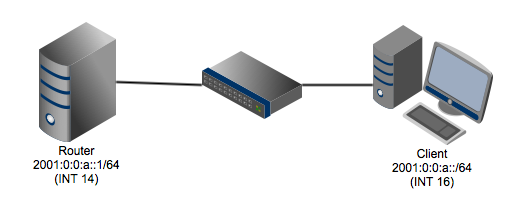
\includegraphics[width=0.90\textwidth]{img/lab04.png}
	\caption{Netzwerktopologie der Übung}
	\label{fig:topologie}
\end{figure}
Ein Ubuntu Rechner fungiert hierbei als eine Art von DHCP Server. Bei IPv6 ist kein DHCP Server mehr notwendig um neuen Clients automatisch eine IP Adresse zuweisen zu können. Allerdings muss auf mindestens einem Rechner der sogenannte Route Advertisement Daemon (radvd) laufen um die Netzwerkkonfiguration im Netz zu verbreiten. Der zweite Rechner ist hierbei nur ein Client der neu ins Netzwerk integriert wird und dabei eine IP Adresse anfordert.

\subsection{Konfiguration des radvd}
Der Route Advertisement Daemon (radvd) ist ein Service der auf dem Rechner läuft und regelmäßig eine Router Advertisement über das Netzwerk schickt um sich neuen Clients bekannt zu machen. Außerdem reagiert er auf Router Solicitation Nachrichten von Clients. Der radvd muss dabei mit den entsprechenden Parametern konfiguriert werden. Listing \ref{lst:radvd.conf} zeigt die radvd.conf des Service auf dem Rechner in der Übung.
\begin{lstlisting}[style=code,caption={radvd.conf},label=lst:radvd.conf]
interface eth1
{
	AdvSendAdvert on;
	AdvIntervalOpt on;
	MinRtrAdvInterval 1;
	MaxRtrAdvInterval 4;
	AdvHomeAgentFlag off;
	prefix 2001:0:0:a::/64
	{
		AdvOnLink on;
		AdvAutonomous on;
		AdvRouterAddr on;
	};
};
\end{lstlisting}
In der ersten Zeile ist der Name des Interfaces (eth1) angegeben auf dem der Service lauscht. In den weiteren Zeilen kann die Router Advertisement an/aus geschalten werden und deren Verbreitungsintervall konfiguriert werden. Die wichtigste Zeile der Konfiguration ist \verb!prefix!. Hier wird konfiguriert welche Netzinformation verbreitet wird. Im Fall dieser Übung handelt es sich um das Netz 2001:0:0:a::/64.
Mittels radvd –C /etc/radvd.conf kann der Service gestartet werden. Der Parameter -C gibt dabei den Ort des Konfigurationsfiles.

TODO: ifconfig des Routers einfügen mir Erklärung.

\section{Neighbour Discovery Protocol Ablauf}
Um einen neuen Ablauf des Protokolls zu initiieren wird das Interface eth1 des Clients, das mt dem Router verbunden ist, neu hochgefahren. Als Erstes wird dabei vom Client eine Router Solicitation Nachricht gesendet um die Konfiguration vom Router zu erhalten. Dieser Antwortet mit einer Router Advertisement Nachricht an den Client. Daraufhin baut sich der Client aus den nun bekannten Präfixen aus der Router Advertisement Nachricht und seiner Hardwareadresse des Interfaces eine IP Adresse zusammen. Daraufhin sendet der Client eine Neighbor Solicitation an alle Clients im Netzwerk. Sofern kein anderer Rechner mit einer Neighbor Advertisement antwortet, so weis der ursprüngliche Client, dass diese Adresse frei ist und kann diese ab sofort benutzen.

\textbf{TODO: Einfügen von Wireshark mitgesnifftem}

Nach erfolgreicher Durchführung des Neighbour Discovery Protocols kann mit dem Befehl \verb!ifconfig! die Konfiguration überprüft werden. Listing \ref{lst:client:ipconfig} zeigt die IP Konfiguration des Clients nach der Durchführung.
\begin{lstlisting}[style=code,caption={IP Konfiguration des Clients},label=lst:client:ipconfig]
root@U460-16:/home/its# ifconfig
eth1  Link encap:Ethernet  HWaddr d8:d3:85:77:23:81  
      inet6 addr: 2001::a:dad3:85ff:fe77:2381/64 Scope:Global
      inet6 addr: fe80::dad3:85ff:fe77:2381/64 Scope:Link
      inet6 addr: 2001::a:a8b7:a9b:a367:3544/64 Scope:Global
      UP BROADCAST RUNNING MULTICAST  MTU:1500  Metric:1
      RX packets:849 errors:0 dropped:0 overruns:0 frame:0
      TX packets:428 errors:0 dropped:0 overruns:0 carrier:0
      collisions:0 txqueuelen:1000 
      RX bytes:132118 (132.1 KB)  TX bytes:82430 (82.4 KB)
      Interrupt:19 Memory:f0400000-f0420000  
\end{lstlisting}
Hier erkennt man, dass der Client sich nun die IP Adresse 2001::a:dad3:85ff:fe77:2381/64 mittels Autokonfiguration zugewiesen hat. Diese enthält dabei das vom Router verbreitete Prefix 2001:0:0:a::/64.
Anschließend konnten sich der Router und der Client über diese IPv6 Adressen gegenseitig erreichen. Überprüft wurde das durch einen Ping-Versuch.

\section{Fragen}

\subsection{Welche Nachrichten stehen im Neighbour Discovery Protocol zur Verfügung?}
Das NDP nutz ICMPv6 um die Informationen im Netzwerk auszutauschen. Es definiert dabei folgende 5 verschiedene Nachrichten.
\begin{itemize}
\item \textbf{Router Solicitation:} Mittles dieser Nachricht werden von Clients eine Router Advertisement von allen Routern im Netzwerk angefordert.
\item \textbf{Router Advertisement:} Damit antworten Router auf Router Solicitation Nachrichten um die IP Konfiguration im Netzwerk zu verteilen. Neben den Antworten auf Router Solicitation Nachrichten senden Router diese Nachricht auch periodisch ins Netzwerk.
\item \textbf{Neighbor Solicitation:} Damit testen Clients ihre ausgewählten IP Adressen im Netzwerk ob diese auch eindeutig sind oder bereits vergeben. Bekommen Clients keine Antwort auf ihre Neighbor Solicitation Nachricht so nehmen sie ihre Adresse als gültig an.
\item \textbf{Neighbor Advertisement:} Diese Nachricht wird gesendet falls ein Client bereits die IP Adresse besitzt die ein anderer Client über eine Neighbor Solicitation Nachricht verbreitet. Damit wird dem neuen Client bekannt gemacht, dass er eine andere IP Adresse wählen muss.
\item \textbf{Redirect:} Mittels einer Redirect Nachricht können Router bessere Routen bekannt geben sofern es einen anderen besseren ersten Hop gibt zu gewissen Zielen.
\end{itemize}

\subsection{Welche Nachrichten in der IPv4 Welt werden dadurch das NDP IPv6 ersetzt?}
Das NDP von IPv6 ersetzt mit seinen verfügbaren Nachrichten das Address Resolution Protocol (ARP) von IPv4. Dabei verwaltet jeder Client eigene Address-Caches bei dem zu jeder IPv6-Adresse eine Link-Layer Adresse steht. Die Link-Layer Adressen von Clients werden dabei über Neighbor-Solicitation-Nachrichten erfragt.

\subsection{Wie funktioniert der Address Autoconfiguration Mechanismus?}
Als allererstes konfiguriert sich der Client eine Link-local-Adresse die er aus dem Prefix FE80 und seinem Interface Indentifier zusammenbaut. Danach generiert der Client die Solicited-Node Multicast Adresse und sendet eine Neighbor Solicitation Nachricht an die Solicited-Node Multicast Adresse. Sofern kein Client antwortet ist diese Adresse nicht vergeben und kann vom ursprünglichen Client verwendet werden. Ist dieser Fall eingetreten sendet der Client anschließend eine Router Solicitation Nachricht an alle Router (FE02::2) um die Netzwerkinformationen zu erhalten. Mit den Informationen aus der Router Advertisement Nachricht kann sich der Client nun eine Global Unicast Adresse konfigurieren und ist nun bereit im Internet zu kommunizieren. 

\subsection{Erläutern Sie den Neighbour Unreachability Detection Mechanismus?}
Der Neighbour Unreachability Detection Mechanismus ist Teil des Neighbour Discovery Protocols und wird verwendet um die Adress-Caches der Clients auf dem neuesten Stand zu halten. Sofern regelmäßig mit einem Client kommuniziert wird ist die Neighbour Unreachability Detection nicht notwendig. Überschreitet ein Eintrag im Adress-Cache allerdings seinen Gültigkeitszeitraum ohne das eine Kommunikation stattgefunden hat, so wird überprüft ob der Client noch verfügbar ist. Zuerst wird versucht die Erreichbarkeit des anderen Clients mittels normaler Kommunikation zu bestätigen. Antwortet dieser nicht so wird anschließend eine Neighbor-Solicitation-Nachricht für diesen Client versendet. Erhält der Client wieder keine Antwort so wird der Kommunikationspartner aus dem Adress-Cache entfernt.

\subsection{Wie wird eine Duplicate Address Detection durchgeführt? Wer ist daran beteiligt?}
Die Duplicate Address Detection ist Teil des Neighbor Discovery Protocols und wird bei der Address Autoconfiguration verwendet. Während der Address Autokonfiguration muss der Client überprüfen ob die von ihm gewählte Adresse noch frei ist. Dazu sendet er eine Neighbor Solicitation Nachricht an die vorher generierte Solicited-Node Multicast Adresse. Antwortet ihm daraufhin ein anderer Client mit einer Neighbor Advertisement Nachricht auf der All-Nodes Multicast Adresse so ist diese Adresse bereits vergeben und es muss eine manuelle Konfiguration vorgenommen werden. Erhält der Client hingegen keine Antwort so gilt die gewählte Adresse als nicht vergeben und kann vom Client verwendet werden. An der Duplicate Address Detection sind somit alle Clients am selben Link beteiligt.

\subsection{Welche Sicherheitsrisiken bestehen bei NDP IPv6?}
Wie beim DHCP-Spoofing können Clients im Netzwerk nicht kontrollieren von wem die Informationen gesendet werden und ob diese korrekt sind oder verfälscht. Ein Angreifer kann sich demnach, sofern er sich bereits im Netzwerk befindet, als Router ausgeben und gefälschte IP Konfigurationen im Netzwerk verbreiten. 
Außerdem kann ein Angreifer feststellen welche IP Adressen im Netzwerk bereits verwendet sind und auch auf Neighbor Solicitation Nachrichten mit gefälschten Neighbor Advertisement antworten.

\subsection{Wie kann die Sicherheit verbessert werden? }
Für das NDP gibt es eine Erweiterung namens SEND (SEcure Neighbor Discovery). Dieses erweitert das NDP um einen Sicherheitsmechanismus der auf Zertifikaten und einer Public-Key-Infrastrutur basiert. Dabei dürfen nur mehr Router eine Konfiguration im Netzwerk verbreiten die sich über ein Zertifikat ausweisen können. Dieses Zertifikat wird dabei von den Clients überprüft bevor sie die Konfiguration annehmem.  

\newpage
%----------------------------------------------------------------------------------------
%	APPENDICES
%----------------------------------------------------------------------------------------
\begin{appendix}
\end{appendix}

%----------------------------------------------------------------------------------------
%	LISTS
%----------------------------------------------------------------------------------------
% List of Figures
\newpage
\phantomsection
\addcontentsline{toc}{section}{\listfigurename}
\listoffigures

% List of Tables
%\newpage
%\phantomsection
%\addcontentsline{toc}{section}{\listtablename}
%\listoftables

% List of Listings
%\newpage
\phantomsection
\addcontentsline{toc}{section}{\lstlistlistingname}
\lstlistoflistings

% Bibliography
%\newpage
%\phantomsection
%\addcontentsline{toc}{section}{Literatur}
%\bibliographystyle{plain}
%\bibliography{bibliography}

%----------------------------------------------------------------------------------------

\end{document}
